\documentclass[journal,12pt,onecolumn]{IEEEtran}

% Import necessary packages
\usepackage{cite}
\usepackage{amsmath,amssymb,amsfonts,amsthm}
\usepackage{algorithmic}
\usepackage{graphicx}
\usepackage{textcomp}
\usepackage{xcolor}
\usepackage{txfonts}
\usepackage{listings}
\usepackage{enumitem}
\usepackage{mathtools}
\usepackage{gensymb}
\usepackage{comment}
\usepackage[breaklinks=true]{hyperref}
\usepackage{tkz-euclide} 
\usepackage{listings}
\usepackage{gvv}                                        
\usepackage[latin1]{inputenc}                                
\usepackage{color}                                            
\usepackage{array}                                            
\usepackage{longtable}                                       
\usepackage{calc}                                             
\usepackage{multirow}                                         
\usepackage{hhline}                                           
\usepackage{ifthen}                                           
\usepackage{lscape}
\usepackage{tabularx}
\usepackage{array}
\usepackage{float}
\usepackage{multicol} % Add the multicol package

% New theorem declarations
\newtheorem{theorem}{Theorem}[section]
\newtheorem{problem}{Problem}
\newtheorem{proposition}{Proposition}[section]
\newtheorem{lemma}{Lemma}[section]
\newtheorem{corollary}[theorem]{Corollary}
\newtheorem{example}{Example}[section]
\newtheorem{definition}[problem]{Definition}

% Custom command definitions
\newcommand{\BEQA}{\begin{eqnarray}}
\newcommand{\EEQA}{\end{eqnarray}}
\newcommand{\define}{\stackrel{\triangle}{=}}

\theoremstyle{remark}
\newtheorem{rem}{Remark}

% Document begins here
\begin{document}
\bibliographystyle{IEEEtran}
\vspace{3cm}

% Title of the document
\title{ASSIGNMENT 1}
\author{EE24BTECH11011 - PRANAY}
\maketitle

\bigskip

% Custom figure and table numbering
\renewcommand{\thefigure}{\theenumi}
\renewcommand{\thetable}{\theenumi}
\begin{enumerate}
    \item The common emmiter forward current gain of the transistor shown is $\beta_F = 100$
	    \begin{center}
% Include the second PDF
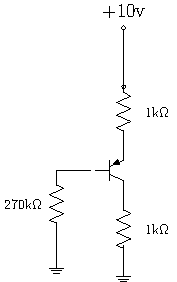
\includegraphics[width=0.2\textwidth]{figs/fig1/main} % Only the base name is specified
\end{center}
The transistor is operating in
 

\begin{enumerate}
    \item saturation region
    \item cutoff region
    \item reverse active region
    \item forward active region\\
\end{enumerate}
    \item The three terminal linear voltage regulator is connected to a $10 \ohm$ load resistor as shown in the figure.If $V_{\text{in}}$ is $10 V$ , what is the power dissipated in the transistor?
	     \begin{center}
% Include the second PDF
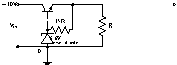
\includegraphics[width=0.5\textwidth]{figs/fig2/main} % Only the base name is specified
\end{center}

    \begin{enumerate}
        \item $0.6 W$
        \item $2.4 W$
        \item $4.2 W$
        \item $5.4 W$\\
    \end{enumerate}
    \item Consider the transformer connections is a part of a power system shown in the figure.The nature of the transformer connections and phase shifts are indicated for all but one transformer.
    Which of the following connections,and the corresponding phase shift $\theta$ , should be used for the transformer between $\mathbf{A}$ and $\mathbf{B}$?
		 \begin{center}
% Include the second PDF
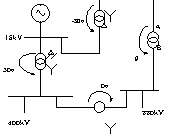
\includegraphics[width=0.5\textwidth]{figs/fig3/main} % Only the base name is specified
\end{center}

    \begin{enumerate}
        \item Star - Star $\brak{\theta = 0\degree}$
        \item Star - Delta $\brak{\theta = -30\degree}$
        \item Delta - Star $\brak{\theta = 30\degree}$
        \item Star - Zigzag $\brak{\theta = 0\degree}$\\
    \end{enumerate}
    \item The incremental cost curves in Rs/M Whr for two generators supplying a common load of $700$MW are shown in the figures.The maximum and minimum generation limits are also indicated.The optimum generation schedule is $\colon$
	     \begin{center}
% Include the second PDF
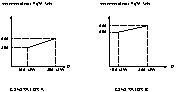
\includegraphics[width=0.8\textwidth]{figs/fig4/main} % Only the base name is specified
\end{center}

    \begin{enumerate}
        \item Generator $\mathbf{A} \colon 400$MW, Generator $\mathbf{B} \colon 300$MW
         \item Generator $\mathbf{A} \colon 350$MW, Generator $\mathbf{B} \colon 350$MW
          \item Generator $\mathbf{A} \colon 450$MW, Generator $\mathbf{B} \colon 250$MW
           \item Generator $\mathbf{A} \colon 425$MW, Generator $\mathbf{B} \colon 275$MW\\
    \end{enumerate}
    \item Two regional systems, each having several synchronous generators and loads are interconnected by an ac line and a HVDC link as shown in the figure. Which of the following statements is true in the steady state:
	     \begin{center}
% Include the second PDF
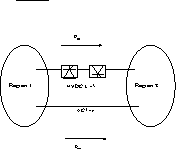
\includegraphics[width=0.5\textwidth]{figs/fig5/main} % Only the base name is specified
\end{center}

\begin{enumerate}
    \item  Both regions need not have the same frequency 
\item The total power flow between the regions $P_{ac} + P_{dc}$ can be changed by controlling the HVDC converters alone 
\item The power sharing between the ac line and the HVDC link can be changed by controlling the HVDC converters alone 
\item The direction of power flow in the HVDC link $P_{dc}$ cannot be reversed.\\
\end{enumerate}
\item Consider a bundled conductor of an overhead line, consisting of three identical sub-conductors placed at the corners of an equilateral triangle as shown in the figure. If we neglect the charges on the other phase conductors and ground, and assume that spacing between sub-conductors is much larger than their radius, the maximum electric field intensity is experienced at
	 \begin{center}
% Include the second PDF
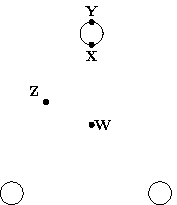
\includegraphics[width=0.5\textwidth]{figs/fig6/main} % Only the base name is specified
\end{center}

\begin{enumerate}
    \item Point $X$
     \item Point $Y$
      \item Point $Z$
       \item Point $W$\\
\end{enumerate}
\item The circuit shown in the figure is
 \begin{center}
% Include the second PDF
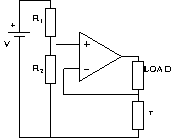
\includegraphics[width=0.5\textwidth]{figs/fig7/main} % Only the base name is specified
\end{center}

\begin{enumerate}
    \item a voltage source with voltage $\frac{rV}{R_1 // R_2}$\\
    \item a voltage source with voltage $\frac{r//R_2}{R_1}V$\\
    \item a current source with current $\frac{r//R_2}{R_1 + R_2}\frac{V}{r}$\\
    \item a current source with current $\frac{R_2}{R_1 + R_2}\frac{V}{r}$
\end{enumerate}
\item The system shown in the figure is
	 \begin{center}
% Include the second PDF
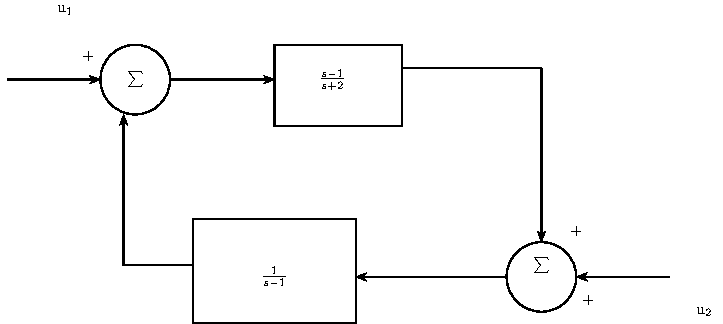
\includegraphics[width=0.8\textwidth]{figs/fig10/main} % Only the base name is specified
\end{center}
\begin{enumerate}
    \item stable
    \item unstable
    \item conditionally stable
    \item stable for output $u_1$ but unstable for input $u_2$\\
\end{enumerate}
\item Let a signal $a_1 \sin\brak{\omega_1 t + \phi_1}$ be applied to a stable linear time-invariant system. Let the corresponding steady state output be represented as $a_2 F\brak{\omega_2 t + \phi_2}$. Then which of the following statements is true?

\begin{enumerate}
    \item$F$ is not necessarily a "sine" or "cosine" function but must be periodic with $\omega_1 = \omega_2$.
    \item $F$ must be a "sine" or "cosine" function with $a_1 = a_2$.
    \item $F$ must be a "sine" function with $\omega_1 = \omega_2$ and $\phi_1 = \phi_2$.
    \item $F$ must be a "sine" or "cosine" function with $\omega_1 = \omega_2$.\\
\end{enumerate}
\item The frequency spectrum of a signal is shown in the figure.If this signal is ideally sampled at intervals of $1$ ms,then the frequency of the sampled signal will be
	 \begin{center}
% Include the second PDF
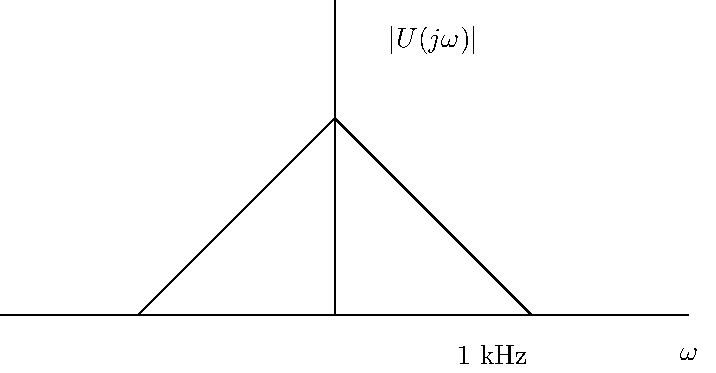
\includegraphics[width=0.5\textwidth]{figs/fig8/Fig8.1/main} % Only the base name is specified
\end{center}
	
\begin{enumerate}
    \item	 \begin{center}
% Include the second PDF
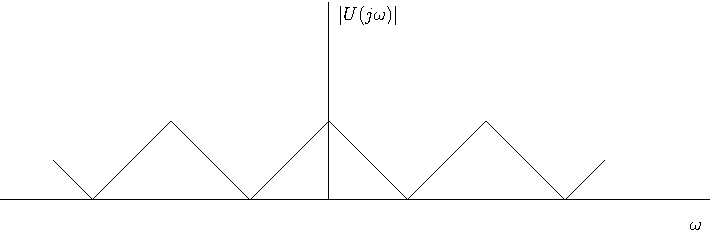
\includegraphics[width=0.5\textwidth]{figs/fig8/fig8.2/main} % Only the base name is specified
\end{center}
 
    \item 	 \begin{center}
% Include the second PDF
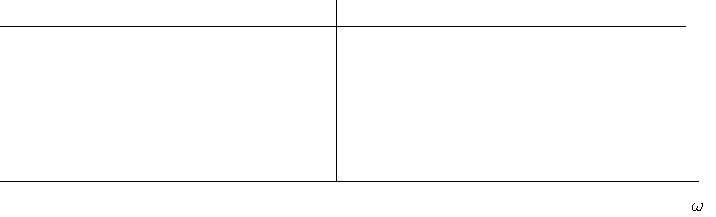
\includegraphics[width=0.5\textwidth]{figs/fig8/fig8.3/main} % Only the base name is specified
\end{center}

    \item 	 \begin{center}
% Include the second PDF
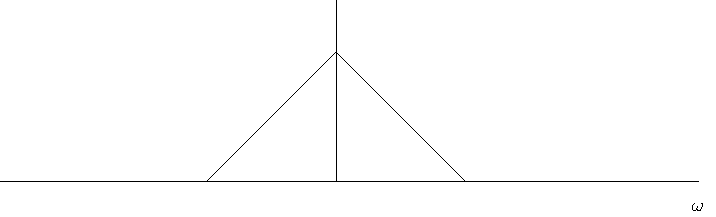
\includegraphics[width=0.5\textwidth]{figs/fig8/fig8.4/main} % Only the base name is specified
\end{center}

    \item 	 \begin{center}
% Include the second PDF
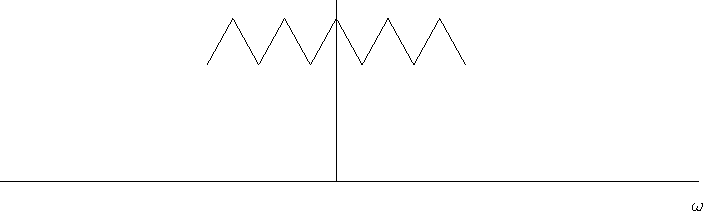
\includegraphics[width=0.5\textwidth]{figs/fig8/fig8.5/main} % Only the base name is specified
\end{center}\\

\end{enumerate}
\item Divergence of the vector field 
\begin{align}
    \vec{A}\brak{x,y,z} = -\brak{x \cos{xy}+y}\vec{i} + \brak{y \cos{xy}}\vec{j} + \brak{\sin{z^2}+x^2+y^2}\vec{k}
\end{align}
is
\begin{enumerate}
    \item $2z \cos{z^2}$
    \item $\sin{xy}+2z\cos{z^2}$
    \item $x\sin{xy}-\cos{z}$
    \item none of these\\
\end{enumerate}
\item $\vec{x} = \sbrak{x_1 x_2 \dots x_n}^\top$ is a $n - $ multiple non-zero vector.Then $n\times n$ matrix $\vec{V} = \vec{x}\vec{x}^\top$
\begin{enumerate}
    \item has rank zero
    \item has rank $1$
    \item is orthogonal
    \item has rank $n$
\end{enumerate}
\item A single-phase fully controlled thyristor bridge ac-dc converter is operating at a firing angle of $25\degree$ and an overlap of angle $10\degree$ with a cnstant dc output of $20\text{A}$.The fundamental power factor(displacement current) at input ac mains is
\begin{enumerate}
    \item $0.78$
    \item $0.827$
    \item $0.866$
    \item $0.9$
\end{enumerate}
\item  A three-phase, fully-controlled thyristor bridge converter is used as line commutated
inverter to feed $50$ kW power at $420$ V dc to a three-phase, $415$ V (line), $50$ Hz ac
mains. Consider dc link current to be constant. The rms current of the thyristor is 
\begin{enumerate}
\item $119.05$ A  \item $79.37$ A \item $68.73$ A 
\item $39.68 A$
\end{enumerate}
    \item In a transformer, zero voltage regulation at full load is 
    \begin{enumerate}
\item not possible 
\item possible at unity power factor load 
\item possible at leading power factor load 
\item possible at lagging power factor load\\
\end{enumerate}
\item The dc motor, which can provide zero speed regulation at full load without any
controller, is 
\begin{enumerate} \item series \item shunt \item cumulative compound \item differential compound\\
\end{enumerate}
\item  The probes of a non-isolated, two-channel oscilloscope are clipped to points A, B, and C in the circuit of the adjacent figure. $V_{\text{in}}$ is a square wave of a suitable low frequency. The display on $\text{Ch}_1 $ and $\text{Ch}_2$ are as shown on the right. Then the Signal and Ground probes $ S_1, G_1 $ and $ S_2, G_2 $ of $ \text{Ch}_1 $ and $ \text{Ch}_2 $respectively are connected to points: 
		 \begin{center}
% Include the second PDF
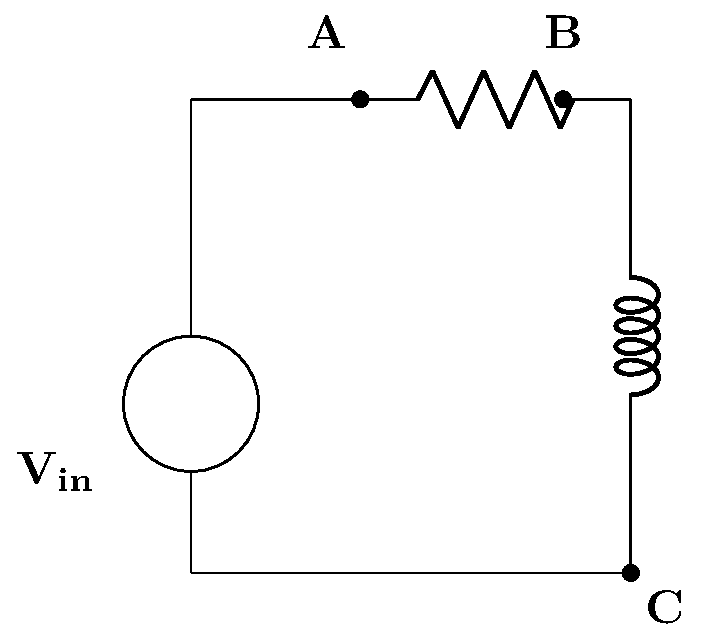
\includegraphics[width=0.4\textwidth]{figs/fig9/fig9.1/main} % Only the base name is specified
\end{center}
	 \begin{center}
% Include the second PDF
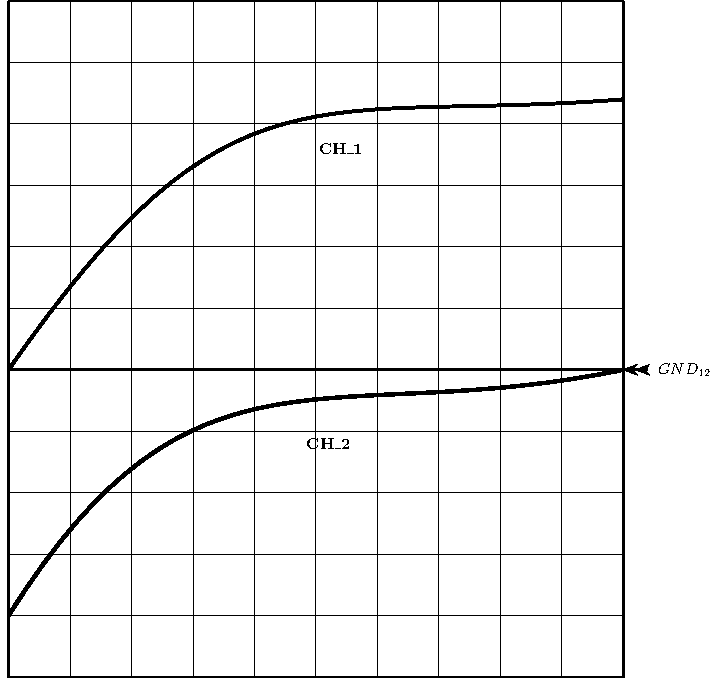
\includegraphics[width=0.4\textwidth]{figs/fig9/9.2/main} % Only the base name is specified
\end{center}


\begin{enumerate}
    \item A, B, C, A
    \item A, B, C, B
    \item C, B, A, B
    \item B, A, B, C
\end{enumerate}
\end{enumerate}

\end{document}
